
% v2-acmsmall-sample.tex, dated March 6 2012
% This is a sample file for ACM small trim journals
%
% Compilation using 'acmsmall.cls' - version 1.3 (March 2012), Aptara Inc.
% (c) 2010 Association for Computing Machinery (ACM)
%
% Questions/Suggestions/Feedback should be addressed to => "acmtexsupport@aptaracorp.com".
% Users can also go through the FAQs available on the journal's submission webpage.
%
% Steps to compile: latex, bibtex, latex latex
%
% For tracking purposes => this is v1.3 - March 2012
\documentclass[prodmode,acmtecs]{acmsmall} % Aptara syntax
\usepackage[spanish,polish]{babel}
\usepackage[T1]{fontenc}
\usepackage{fancyvrb}
\usepackage{graphicx,hyperref}
\newcommand\cutout[1]{}


\usepackage[table]{xcolor}
\usepackage[utf8]{inputenc}
\usepackage[parfill]{parskip}
\usepackage{tabulary}
\PassOptionsToPackage{hyphens}{url}
\usepackage{hyperref}    
\usepackage[capitalize]{cleveref}


% Metadata Information
% !!! TODO: SET THESE VALUES !!!
\acmVolume{0}
\acmNumber{0}
\acmArticle{CFP}
\acmYear{0}
\acmMonth{0}

\newcounter{colstart}
\setcounter{page}{4}

\RecustomVerbatimCommand{\VerbatimInput}{VerbatimInput}%
{
%fontsize=\footnotesize,
fontfamily=\rmdefault
}


\newcommand{\UnderscoreCommands}{%\do\verbatiminput%
\do\citeNP \do\citeA \do\citeANP \do\citeN \do\shortcite%
\do\shortciteNP \do\shortciteA \do\shortciteANP \do\shortciteN%
\do\citeyear \do\citeyearNP%
}

\usepackage[strings]{underscore}



% Document starts
\begin{document}


\setcounter{colstart}{\thepage}

\acmArticle{CFP}
\title{\huge\sc SIGLOG Monthly 216}
\author{DAVID PURSER\affil{Max Planck Institute for Software Systems, Saarbr\"ucken}
\vspace*{-2.6cm}\begin{flushright}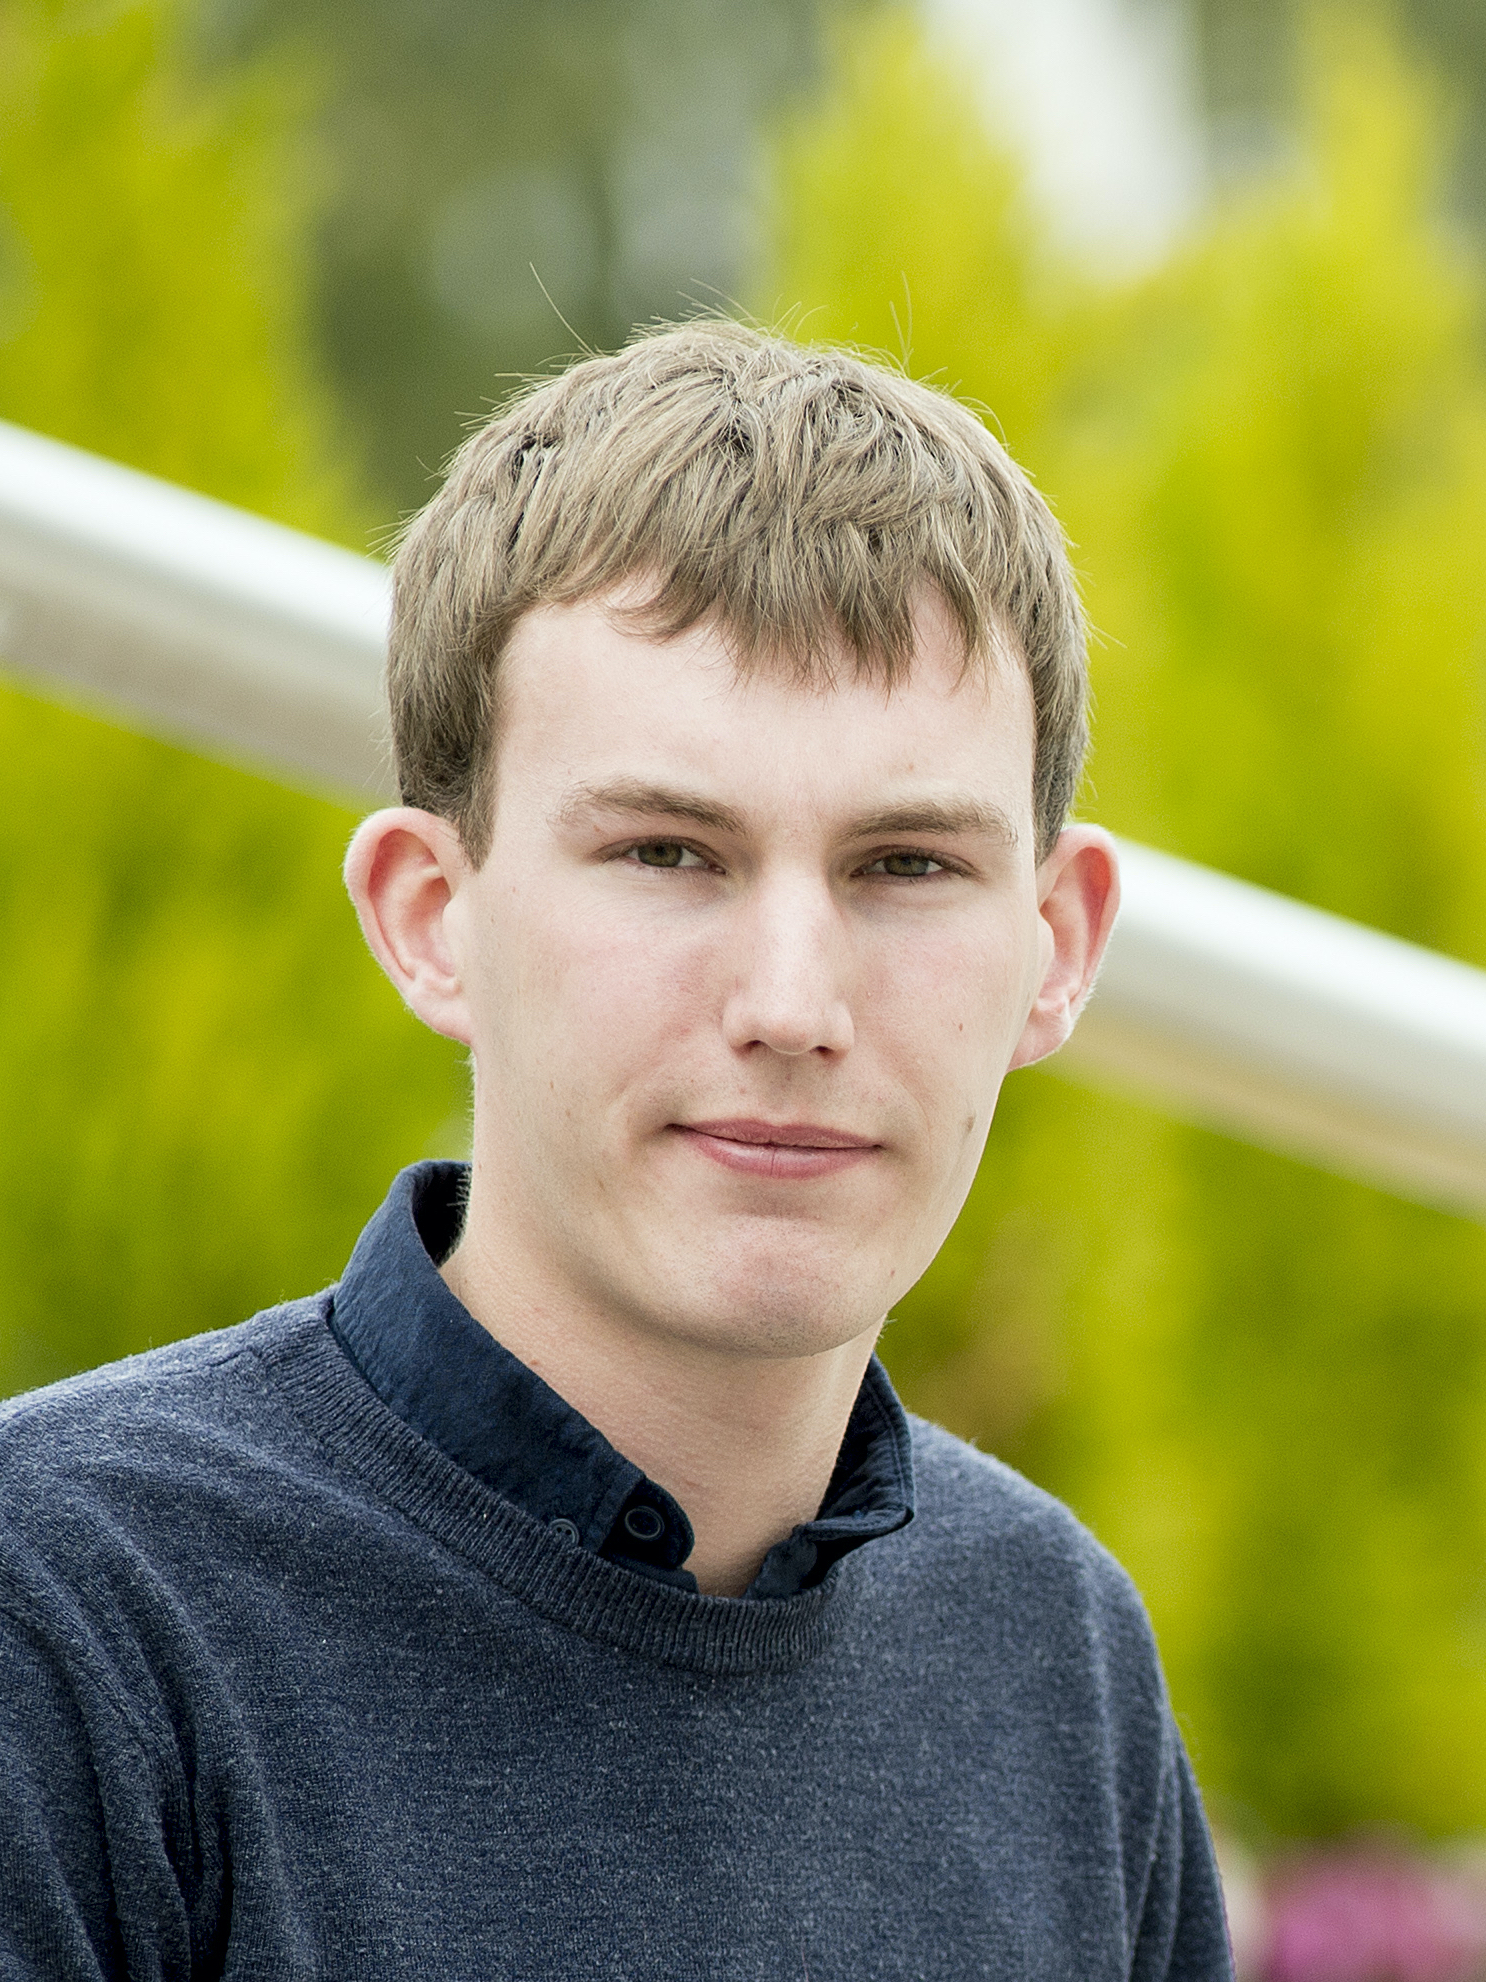
\includegraphics[width=30mm]{dp}\end{flushright}
}

\maketitlee

\href{https://lics.siglog.org/newsletters/}{Past Issues}
 - 
\href{https://lics.siglog.org/newsletters/inst.html}{How to submit an announcement}
\section{Table of Content}\begin{itemize}\item DEADLINES (\cref{deadlines}) 
 
\item CALLS 
 
\begin{itemize}\item MEandE-LP 2021 (CALL FOR PAPERS) (\cref{MEandELP2021})
\item MFCS 2021 (CALL FOR PARTICIPATION) (\cref{MFCS2021})
\item FORMATS 2021 (CALL FOR PARTICIPATION) (\cref{FORMATS2021})
\item PM 2021 (CALL FOR PARTICIPATION) (\cref{PM2021})
\item ICGI2020 (CALL FOR PARTICIPATION) (\cref{ICGI2020})
\end{itemize} 
\item JOB ANNOUNCEMENTS 
 
\begin{itemize}\item Tenure track lecturer (Research) “Static security guarantees for programming languages”, Vrije Universiteit Brussel (\cref{TenuretracklecturerResearchStaticsecurityguaranteesforprogramminglanguagesVrijeUniversiteitBrussel})
\end{itemize} 
\end{itemize}\section{Deadlines}\label{deadlines}\rowcolors{1}{white}{gray!25}\begin{tabulary}{\linewidth}{LL}MEandE-LP 2021:  & Aug 02, 2021 (Paper) \\
MFCS 2021:  & Aug 07, 2021 (Early registration deadline) \\
FORMATS 2021:  & Aug 20, 2021 (Registration deadline) \\
PM 2021:  & Aug 20, 2021 (Registration deadline) \\
ICGI2020:  & August 23, 2021 (Start of conference) \\
RW 2021:  & Aug 25, 2021 (Registration closes) \\
CCC 2021:  & Aug 30, 2021 (Deadline) \\
Tenure track lecturer (Vrije Universiteit Brussel):  & Sept 6, 2021 (application deadline) \\
CPP 2022:  & Sep 16, 2021 (Abstract Submission Deadline) \\
FLoC 2022:  & Sep 27, 2021 (Submission of workshop proposals deadline) \\
\end{tabulary}
\section{MEandE-LP 2021: 1st Workshop on Machine Ethics and Explainability-The Role of Logic Programming }\label{MEandELP2021}  \href{https://sites.google.com/view/meande2021}{https://sites.google.com/view/meande2021}\\ 
  September 20-21, 2021 (ICLP Workshop) \\ 
  Fully virtual event hosted by the Department of Computer Science of the University of Porto. \\ 
CALL FOR PAPERS 

\begin{itemize}\item  INVITED SPEAKERS 
 
\begin{itemize}\item  Luis Moniz Pereira, New University of Lisbon, Portugal.
\item  Francesca Toni, Imperial College of London, UK.                      
\end{itemize} 
\item  AIMS AND SCOPE 
 
  Machine Ethics, Explainability are two recent topics that have been attracting a lot of attention and concern in the last years. This global concern has manifested in many initiatives at different levels. There is an intrinsic relation between these two topics. It is not enough for an autonomous agent to behave ethically, it should also be able to explain its behavior, i.e. there is a need for both ethical component and explanation component. Furthermore, an explainable behavior is obviously not acceptable if it is not ethical (i.e., does not follow the ethical norms of the society). 
 
  In many application domains especially when human lives are involved (and ethical decisions must be made), users need to understand well the system recommendations, to be able to explain the reasons for their decisions to other people. One of the most important ultimate goals of explainable AI systems is the efficient mapping between explainability and causality. Explainability is the system ability to explain itself in natural language to average user by being able to say, ``I generated this output because x,y,z''. In other words, the ability of the system to state the causes behind its decision is central for explainability.  
 
  However, when critical systems (ethical decisions) are concerned, is it enough to explain system's decisions to the human user? Do we need to go beyond the boundaries of the predictive model to be able to observe a cause and effect within the system? 
 
  There exists a big corpus of research work on explainability, trying to explain the output of some blackbox model following different approaches. Some of them try to generate logical rules as explanations. However, it is worth noting that most methods for generating post-hoc explanations are themselves based on statistical tools, that are subject to uncertainty or errors. Many of the post-hoc explainability techniques try to approximate deep-learning black-box models with simpler interpretable models that can be inspected to explain the black-box models. However, these approximate models are not provably loyal with respect to the original model, as there are always trade-offs between explainability and fidelity.  
 
  On the other side, a good corpus of researchers has used inherently interpretable approaches to design and implement their ethical autonomous agents. Most of them are based on logic programming, from deontic logics to non-monotonic logics and other formalisms.  
 
  Logic Programming has a great potential in these two emerging areas of research, as logic rules are easily comprehensible by humans, and favors causality which is crucial for ethical decision making.  
 
  Anyway, in spite of the significant amount of interest that machine ethics has received over the last decade mainly from ethicists and artificial intelligence experts, the question ``are artificial moral agents possible?'' is still roaming around. There have been several attempts for implementing ethical decision making into intelligent autonomous agents using different approaches. But, so far, no fully descriptive and widely acceptable model of moral judgment and decision making exists. None of the developed solutions seem to be fully convincing to provide a trusted moral behavior. The same goes for explainability, in spite of the global concern about the explainability of the autonomous agents' behaviour, existing approaches do not seem to be satisfactory enough. There are many questions that remain open in these two exciting, expanding fields. 
 
  This workshop aims to bring together researchers working in all aspects of machine ethics and explainability, including theoretical work, system implementations, and applications. The co-location of this workshop with ICLP is intended also to encourage more collaboration with researchers from different fields of logic programming.This workshop provides a forum to facilitate discussions regarding these topics and a productive exchange of ideas. 
 
\item  TOPICS of interest include (but are not limited to):     
 
\begin{itemize}\item  New approaches to programming machine ethics;    
\item  New approaches to explainability of blackbox models;    
\item  Evaluation and comparison of existing approaches;    
\item  Approaches to verification of ethical behavior;    
\item  Logic programming applications in machine ethics;    
\item  Integrating logic programing with methods for machine ethics;    
\item  Integrating logic programing with methods for explainability.                     
\end{itemize} 
\item  SUBMISSIONS: \href{https://easychair.org/conferences/?conf=meandelp2021}{https://easychair.org/conferences/?conf=meandelp2021} 
 
  The workshop invites two types of submissions:  
 
\begin{itemize}\item  original papers describing original research. 
\item  non-original paper already published on formal proceedings or journals.
\end{itemize} 
 Original papers in Springer LNCS Format  
 
\begin{itemize}\item  regular papers must not exceed 14 pages (including references) 
\item  extended abstract must not exceed 4 pages (excluding references)
\end{itemize} 
 Authors are requested to clearly specify whether their submission is original or not with a footnote on the first page. 
 
\item  IMPORTANT DATES 
 
\rowcolors{1}{white}{gray!25}\begin{tabulary}{\linewidth}{LL}Paper submission:  & Aug 02, 2021 \\
Author Notification:  & Aug 18, 2021 \\
Camera-ready articles due:  & Aug 25, 2021 \\
\end{tabulary}
 
\item  PROCEEDINGS 
 
  Authors of all accepted original contributions can opt for to publish their work on formal proceedings.  Accepted non-original contributions will be given visibility on the workshop web site including a link to the original publication, if already published. 
 
\end{itemize}\section{MFCS 2021: The 46th International Symposium on Mathematical Foundations of Computer Science}\label{MFCS2021}  August 23-27, 2021, Tallinn, Estonia\\ 
  \href{https://compose.ioc.ee/mfcs/}{https://compose.ioc.ee/mfcs/}\\ 
CALL FOR PARTICIPATION 

\begin{itemize}\item  The MFCS conference series has been organised since 1972. Traditionally, the conference moved between the Czech Republic, Slovakia, and Poland, while since 2013, the conference travels around Europe. In 2021, it will come to Tallinn, Estonia. MFCS is a high quality venue for original research in all branches of theoretical computer science. 
 
\item  INVITED SPEAKERS: 
 
\begin{itemize}\item  Amina Doumane (ENS Lyon)
\item  Martin Grohe (RWTH Aachen University)
\item  Joël Ouaknine (Max Planck Institute for Software Systems)
\item  Eva Rotenberg (Technical University of Denmark)
\item  Barna Saha (UC Berkeley)
\end{itemize} 
\item  The event will be hybrid, both physical and online. Please check the information regarding the programme and the invited speakers at \href{https://compose.ioc.ee/mfcs/}{https://compose.ioc.ee/mfcs/} 
 
\item  REGISTRATION 
 
Early registration deadline: Aug 07, 2021 
 
  Last minute registration is possible, but more expensive. Registration can be done on the website of the conference: \href{https://compose.ioc.ee/mfcs/registration.php}{https://compose.ioc.ee/mfcs/registration.php} 
 
\end{itemize}\section{FORMATS 2021: Formal Modeling and Analysis of Timed Systems  }\label{FORMATS2021}  August 24-26, 2021, Online (Workshops on August 23 and 28, 2021)\\ 
  Part ot QONFEST 2021 August 24-27, 2021\\ 
  \href{https://qonfest2021.lacl.fr/formats21.php}{https://qonfest2021.lacl.fr/formats21.php}\\ 
CALL FOR PARTICIPATION 

\begin{itemize}\item  FORMATS 2021 is an annual conference aimed at promoting the study of fundamental and practical aspects of timed systems,  and bringing together researchers from different disciplines that share interests in modelling, design, and analysis of timed computational systems.  
 
  The conference aims to attract researchers interested in real-time issues in hardware design, performance analysis, real-time software,  scheduling, semantics and verification of real-timed, hybrid and probabilistic systems.   This year's programme includes a special session on control synthesis and motion planning for cyber-physical and control systems, chaired by Morteza Lahijanian. 
 
\item  Invited Speakers at FORMATS 2021:   
 
\begin{itemize}\item  Daniele Magazzeni, King's College, London \& JP Morgan AI Research, UK  
\item  Jana Tumova, KTH Royal Institute of Technology, Stockholm, Sweden  
\end{itemize} 
\item  In 2021 FORMATS is co-organized together with CONCUR 2021, FMICS 2021, QEST 2021, and satellite workshops  Express/SOS 2021, PM 2021, SNR 2021, TRENDS 2021, under the QONFEST 2021 umbrella conference.  
 
  See \href{https://qonfest2021.lacl.fr/}{https://qonfest2021.lacl.fr/} 
 
\item  REGISTRATION 
 
  Registration is free but mandatory.   
 
Registration deadline: Aug 20, 2021 
 
  \href{https://qonfest2021.lacl.fr/registration.php}{https://qonfest2021.lacl.fr/registration.php} 
 
  Depending on the evolution of the pandemic in the Paris region, we will try to hold some physical event, if you are interested please indicate it in the registration form. 
 
\end{itemize}\section{PM 2021: First Workshop on Predictive Maintenance}\label{PM2021}  August 28, 2021, Online, part of QONFEST\\ 
  \href{https://sites.google.com/utwente.nl/pm-2021}{https://sites.google.com/utwente.nl/pm-2021}\\ 
CALL FOR PARTICIPATION 

\begin{itemize}\item  WORKSHOP 
 
  We are happy to invite you to the first workshop in predictive maintenance, co-located with CONCUR @ QONFEST'21. Predictive maintenance is an upcoming field, aiming at optimizing asset maintenance strategies through sensor technology, data analysis, (stochastic) techniques, etc. PM 2021 brings together experts from academia and industry, to share their knowledge and experience on the soaring field of predictive maintenance. This includes: 
 
\begin{itemize}\item  model checking approaches, e.g. to optimise component replacement policies
\item  machine learning predictors, to extrapolate load growth and increased repair frequency
\item  examples of applications in company assets and policies, etc.
\end{itemize} 
  PM 2021 features invited talks by experts from both academia and industry. The specific goal is to offer a computer science perspective on the pushing trends of PM for industrial partners, where participants will be able to interact with personalities in the field. 
 
\item  CONFIRMED SPEAKERS: 
 
\begin{itemize}\item  Kim G. Larsen  (Aalborg University, DK)
\item  Alessandro Abate  (University of Oxford, UK)
\item  Nick Oosterhof  (Dutch Railways, NL)
\item  Alessandro Cimatti  (Fondazione Bruno Kessler, IT)
\item  Roberto Manuel Cibils  (INVAP S.E., AR)
\item  Lisandro Jiménez Roa  (University of Twente, NL)
\item  Jaap van Ekris  (Delta Pi, NL)
\end{itemize} 
\item  Participation is free of charge.  
 
Registration deadline: Aug 20, 2021 
 
  \href{https://qonfest2021.lacl.fr/registration.php}{https://qonfest2021.lacl.fr/registration.php} 
 
\end{itemize}\section{ICGI2020: The 15th International Conference on Grammatical Inference}\label{ICGI2020}  \href{https://icgi2020.lis-lab.fr}{https://icgi2020.lis-lab.fr}\\ 
  August 23-27, 2021\\ 
CALL FOR PARTICIPATION 

\begin{itemize}\item  This event will be conducted virtually online and is free with mandatory registration here: \href{https://icgi2020.lis-lab.fr/register/}{https://icgi2020.lis-lab.fr/register/}   
 
\item  It is our pleasure to inform you about ICGI 2020/21, the major forum for presentation and discussion of original research papers on all aspects of grammar learning. ICGI, which has been organized bi-annually since the early nineties, will be held on-line in August 2021 after being postponed due to COVID-19 last year. 
 
   The conference events take place from Monday, August 23 to Friday, August 27 beginning at 8:00 EDT/14:00 CEST/21:00 JST and running for 2 to 3 hours each day. The program also includes invited talks and tutorials, which are presented live. The accepted papers will be presented asynchronously via pre-recorded videos with dedicated question and answer periods held live. 
 
\item  See the webpage for invited speakers and programme: \href{https://icgi2020.lis-lab.fr/speakers/}{https://icgi2020.lis-lab.fr/speakers/} and \href{https://icgi2020.lis-lab.fr/program/}{https://icgi2020.lis-lab.fr/program/} 
 
\end{itemize}\section{Tenure track lecturer (Research) “Static security guarantees for programming languages”, Vrije Universiteit Brussel}\label{TenuretracklecturerResearchStaticsecurityguaranteesforprogramminglanguagesVrijeUniversiteitBrussel}JOB ANNOUNCEMENT 

\begin{itemize}\item   The computer science department of the Vrije Universiteit Brussel is offering a full-time position as professor to reinforce its programming languages and software engineering branch within the subject area of ``Static security guarantees for programming languages''. 
 
  The position is published under the heading: 
 
\begin{itemize}\item  Tenure track lecturer (Research) “Static security guarantees for programming languages” 
\end{itemize} 
  on the university's job offers website at \href{https://jobs.vub.be/job/Elsene-Tenure-track-lecturer-%28Research%29-\&apos;Static-security-guaranties-for-programming-languages\&apos;/687214901/}{https://jobs.vub.be/job/Elsene-Tenure-track-lecturer-%28Research%29-\&apos;Static-security-guaranties-for-programming-languages\&apos;/687214901/} 
 
  You will be offered a tenure track appointment, for an assignment of 1 FTE, for 5 years, with eligibility for tenure in the rank of associate professor (or higher) by the end of this initial period, with planned starting date 01/02/2022.  
 
  The deadline for applying is September 6th, 2021. Applications should reach us through the website. The person to contact for further information is: 
 
  Prof. dr. Wolfgang De Meuter at Wolfgang.De.Meuter@vub.be or on +02/2629.34.81. 
 
\item  Please see job listing for position description: \href{https://jobs.vub.be/job/Elsene-Tenure-track-lecturer-%28Research%29-\&apos;Static-security-guaranties-for-programming-languages\&apos;/687214901/}{https://jobs.vub.be/job/Elsene-Tenure-track-lecturer-%28Research%29-\&apos;Static-security-guaranties-for-programming-languages\&apos;/687214901/}  
 
\end{itemize}


To the \href{http://siglog.org/}{SIGLOG} or \href{https://lics.siglog.org}{LICS} website\end{document}